\chapter{The Real and Complex Number Systems}

The most important definition in this chapter is \textbf{1.10} about the \textit{least-upper-bound property}, or the $\sup$, and the corresponding $\inf$. Without these concepts it's hard to prove anything else, so please pay attention to this definition!

Although you don't have to understand the $\R$ construction from $\Q$ perfectly, it is a good exercise. It is quite set-theory heavy, so if you haven't read \href{https://amzn.to/3MNZ8e7}{\textit{Naive Set Theory} by Paul Halmos}, I would highly recommend give that book a skim.

I thought it was helpful to think the cuts in the construction as subsets of $\Q$ that kinda look like $(-\infty, r)$. This isn't super precise, but it should aid with the understanding quite a bit (the book should honestly include a diagram for this idea).
I believe these cuts are known as \href{https://en.wikipedia.org/wiki/Dedekind_cut}{Dedekind cuts} in the real world.

\section{Exercises}

\bx{
  Suppose they are trivial, then we have
  \ea{
    \item $r+x = q \in \Q$ so $x = q - r \in \Q$ which is a contradiction
    \item $rx = q \in \Q$ so $x = \frac{q}{r} \in \Q$ which is a contradiction
  }
  so we conclude both are irrational.
  \label{ex:1.1}
}

\bx{
  This is the classic $\sqrt{2}$ is irrational proof, but you start with AFSOC $q \in \Q$ such that
  \begin{align*}
    q^2                & = 12                                              \\
    \pa{\frac{m}{n}}^2 & = 12 \tag{$m, n \in \Z$, $m, n$ relatively prime} \\
    m^2                & = 12n^2
  \end{align*}

  Now, $m$ must be a multiple of 3, so let $m = 3k, k \in \Z$.

  \begin{align*}
    m^2 = 9k^2 & = 12n^2
    3k^2       & = 4n^2
  \end{align*}

  and we conclude the same for $n$, which is a contradiction since we assume $\frac{m}{n}$ was represented as a fraction in simplest forms.
}

\bx{
  These are pretty trivial.
}

\bx{
  Pick an arbitrary $x \in E$, then we have $\alpha \leq x$ by lower bound definition and $x \leq \beta$ by upper bound definition.
  Putting these together, we get
  \begin{equation*}
    \alpha \leq x \leq \beta \implies \alpha \leq \beta
  \end{equation*}
}

\bx{
  Let $\alpha = -\sup(-A) \implies -\alpha = \sup(-A)$. Then we know

  \begin{align*}
    -\alpha & > y \tag{$y \in -A$}       \\
    \alpha  & < -y \tag{$y \in -A$}      \\
    \alpha  & < y' \tag{$y' = -y \in A$} \\
  \end{align*}

  Therefore $\alpha$ is a lower bound for $A$. Now, because of the $\sup$ property of $\alpha$ on $-A$, we know $\not\exists \beta$ such that
  \begin{equation*}
    \beta > \alpha \text{ and } \beta < y \text{ for } y \in -A
  \end{equation*}
  which means $\alpha$ is the largest lower bound for $A$ as well, so therefore we conclude $\alpha = \inf(A)$
}

\bx{
  \ea{
    \item I think the idea here is to show that $m/n = p/q$ AFSOC means $p = km, q = kn, k \in \Q$, and then you say
    \begin{align*}
      \pa{b^m}^{\frac{1}{n}} = A \implies b^m             & = A^n \tag{Theorem 1.21}                                \\
      b^{km}                                              & = A^{kn} \tag{Repeatedly multiply both sides $k$ times} \\
      \pa{b^p}^{\frac{1}{q}} = \pa{b^{km}}^{\frac{1}{kn}} & = A
    \end{align*}
    \label{ex:1.6.a}
    \item Substitute fractions in for $r, s$ and you can derive the rest with help from \ref{ex:1.6.a}.
    \item Any $r' \leq r$ will have $b^{r'} \in B(r)$ by definition of $B(r)$. If $r' > r$, then $r' \not\in B(r)$, hence we see that $b^r = \sup B(r)$.
    \label{ex:1.6.c}
    \item Add $B(x)$ and $B(y)$ and use \ref{ex:1.6.c}.
  }
}

\bx{
  \TODO
}

\bx{
  $i^2 = -1 < 0$ so it is not ordered.
}

\bx{
  \TODO but you just run through the definition and verify.
}

\bx{
  \TODO
}

\bx{
  We just have to set $r = \abs{z}$ and divide $z$'s coefficients by $r$ to get $w$. These are unique because $\abs{z}$ is unique.
}

\bx{
  We can use induction to prove this, starting with the $n=2$ case which is given by axioms.
}

\bx{
  Start with triangle inequality and manipulate. I think you sould WLOG $\abs{x} < \abs{y}$ at some point when you try to get the $\abs{x} - \abs{y}$ term, so you can get your inequality.
}

\bx{
  \begin{align*}
    \abs{1+z}^2 + \abs{1-z}^2 & = (1 + z)(1 + \conj{z}) + (1 - z)(1 - \conj{z})               \\
                              & = 1 + z + \conj{z} + z\conj{z} + 1 - z - \conj{z} + z\conj{z} \\
                              & = 4 \tag{$z\conj{z} = 1$}
  \end{align*}

  You can also do this problem geometrically, realizing that $\abs{z} = 1$ means $z$ is on the unit circle in the complex plane, and that
  \begin{equation}
    \abs{1+z}^2 + \abs{1-z}^2 = \abs{1 - (-z)}^2 + \abs{1-z}^2
  \end{equation}
  which means we are finding the sum of square distances of $z, -z$ from $1$ on the complex plane, which, since $z, -z$ are endpoints of a diameter, their sum distances are the sums of squares of two legs of a right triangle with the diameter as the hypotenuse, which has diameter length 2.
  We then conclude their square sums = $2^2 = 4$.

  \begin{figure}[H]
    \centering
    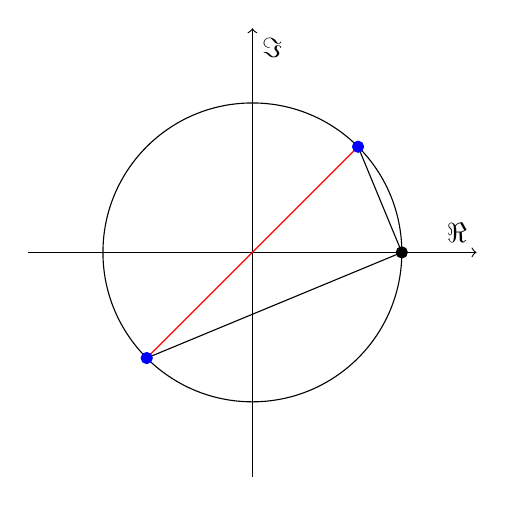
\begin{tikzpicture}
      \begin{axis}[
          ticks=none,
          axis lines = middle,
          axis line style={->},
          ymin=-1.5, ymax=1.5,
          xmin=-1.5, xmax=1.5,
          xlabel={$\Re$},
          ylabel={$\Im$},
          axis equal image
        ]
        \draw (axis cs:0,0) circle [radius=1];
        \addplot[mark=*, only marks] coordinates {(1,0)};
        \addplot[blue, mark=*, only marks] coordinates {
            ({sqrt(2)/2}, {sqrt(2)/2})
            ({-sqrt(2)/2}, {-sqrt(2)/2})
          };
        \draw[red] ({sqrt(2)/2}, {sqrt(2)/2}) --
        ({-sqrt(2)/2}, {-sqrt(2)/2});
        \draw ({sqrt(2)/2}, {sqrt(2)/2}) -- (1,0);
        \draw ({-sqrt(2)/2}, {-sqrt(2)/2}) -- (1,0);
      \end{axis}
    \end{tikzpicture}
    \caption{$z, \conj{z}$ and their square sum distance from 1 is the diameter}
  \end{figure}
}

\bx{
  Taking a look at our derivation, equality would happen when every $\abs{Ba_j - Cb_j} = 0$.
}

\bx{
  \ea{
    \item For some reason I'm only getting $k$ solutions here, since you have the locus of points that are $r$ away from $\bm{x}, \bm{y}$ respectively and you find their intersection.
    \item There is only one point that is equidistant from $\bm{x}$ and $\bm{y}$ and sums up to $d$, which is the midpoint of the two points.
    \item This is impossible because there is no point that can be $<r$ to both points but also cover the $d$ distance.
  }
}

\bx{
  Proving equality is just an algebra exercise, use the conjugate definition.

  Geometrically, we see that $\abs{\bm{x} + \bm{y}}^2 + \abs{\bm{x} - \bm{y}}^2$ are the sum of squares of the diagonals, and the rest are the sums of squares of the side lengths. And we've proved they are equal.
}

\bx{
  In $k=1$ this is not possible because $xy = 0$ implies one of them is 0.

  To some up with a general $\bm{y}$ for any $k$, observe that

  \begin{align*}
    \bm{x} \cdot \bm{y} & = \sum_{i=1}^k x_iy_i                                                                       \\
                        & = x_1 \cdot \frac{1}{x_1} + x_2 \cdot \frac{1}{x_2} + \cdots + x_k \cdot \frac{-(k-1)}{x_k} \\
                        & = k-1 - (k-1) = 0
  \end{align*}

  Geometrically, any perpendicular vector would have a dot product of 0.
}

\bx{
  \TODO
}

\bx{
  \TODO
}